\chapter{Introduction}\label{sec:intro}
\section{Birth of Integrated Circuits}
The development of microelectronics revolutionized the world in the latter half of the twentieth century. The term semiconductor, in the sense it is known today, first appears in literature in 1911 \cite{Koenigsberger_AnnalenDerPhysik1911}. Initially, work on the subject was rather pessimistic. However, in the years following Word War II breakthroughs began shed light on the possible applications and the underlying physics involved, such as the ideas of \emph{instrinsic} and \emph{extrinsic} semiconductors \cite{Busch_EuroJournPhys1989,Lark_AAAS1954,Wilson_Royal1931a,Wilson_Royal1931b}. \\

\noindent The history of semiconductors and transistors is a well documented subject. The first transistor was constructed at Bell Labs in 1947 using polycrystalline germanium. Shortly thereafter one was developed using silicon. Throughout the following years, these devices were improved on by replacing polycrystalline with single crystals \cite{Neamen_Semiconductor_Physics2003}. Then Jack Kilby demonstrated the first  \ac{IC} in 1958, for which he would win the Nobel Prize in physics \cite{Lukasiak_JorunTelcomm2010, Kilby_Patent1959}. The scale of \acp{IC} grew rapidly in the subsequent years. Initially only a few transistors could fit on a chip (small-scale integration), in stark contrast to moder-day chips that contains billions of transistors \cite{Moore_Electronics1965, Clarke_EEtimes2005}. Growth continued at a rapid pace, but eventually it was realized that some limits, material and integration based, existed in silicon and other commonly used materials \cite{Meindl_Science2001, Schulz_Nature1999}. In part, these limitations increased the interest in alternative materials. As a result widespread and renewed interest has led to a breadth information and results on a wide range of materials and their applications.

\section{Graphene as a New \Td Material}\label{sec:graphene}
Layered materials have existed for billions of years, and have been studied over the last few centuries \cite{Golden_EarthSci2013,Brodie_Royal1859}. In recent decades the scientific study of graphite (3D) has led to new forms materials, such as carbon nanotubes (1D) and fullerenes (0D) \cite{Kroto_Nature1985, Balleste_Nanoscale2011,Iijima_Nature1991}. However, only more recently have scientists began to understand the potential of such layered materials and their potential technological applications. After attempting unsuccessfully to synthesize few-layer graphite during the 1960s (only around 10-50 layers were able to be synthesized) a breakthrough was finally acheived \cite{Balleste_Nanoscale2011}. This most notably began with the synthesis of monolayer graphene \cite{Novoselov_Science2004}.

\subsection{Properties of Graphene}\label{subsec:graphene_properties}
To date, graphene's properties have been the focus of much research, both theoretical and experimental. It has been one of the primary driving forces in study of `relativistic' condensed matter physics due to its low dimensionality and its band structure that allows electrons to mimic relativistic particles confirming the appearance of several relativistic phonomena \cite{Geim_NatureMat2007,Geim_Nature2005,Zhang_NatPhys2011,Williams_Science2007}. In its most basic sense, graphene is composed of a single layer of carbon atoms arranged in \td honeycomb lattice (see fig.~\ref{fig:graphene_honeycomb}) It has a Young's modulus of $~100\unita{GPa}$ (several times more than steel) with a breaking force that is $13\%$ of its Young's modulus \cite{Bertolazzi_ACSnano2011, Akinwande_NatureComm2014}. Its stength is due, in part, to its strong in-plane carbon (\ch{C}) bonds. In addition, graphene can sustain elastic deformations of 20\% due to its \td nature and it has high pliability \cite{Balleste_Nanoscale2011}. These mechanical properties are of interest because graphene lies in the extreme ranges of many metrics considering its size and dimensionality.\\

\noindent Aside from its mechanical properties, graphene's transport properties were another reason why the material was so appealing. Graphene's mobility is several times that of silicon's. Experimental results have shown graphene mobility around $15,000\cmvs$ with a potential theoretical limit of $200,000\cmvs$ \cite{Dargys_Encylco1994,Akinwande_NatureComm2014}. The upper theoretical limit imposed on mobility is due to scattering, however, these high mobilities are achieved mainly because electrons in graphene act very much like photons in their mobility due to their lack of mass. This enables them to travel sub-micron distances without scattering \cite{Novoselov_NatureMat2007}. In reality, there are other limiting factors that need to be considered such as the quality of graphene and scattering with the substrate, for example. \\

\begin{figure}[ht]
	\centering
	\begin{minipage}[b]{0.45\linewidth}
		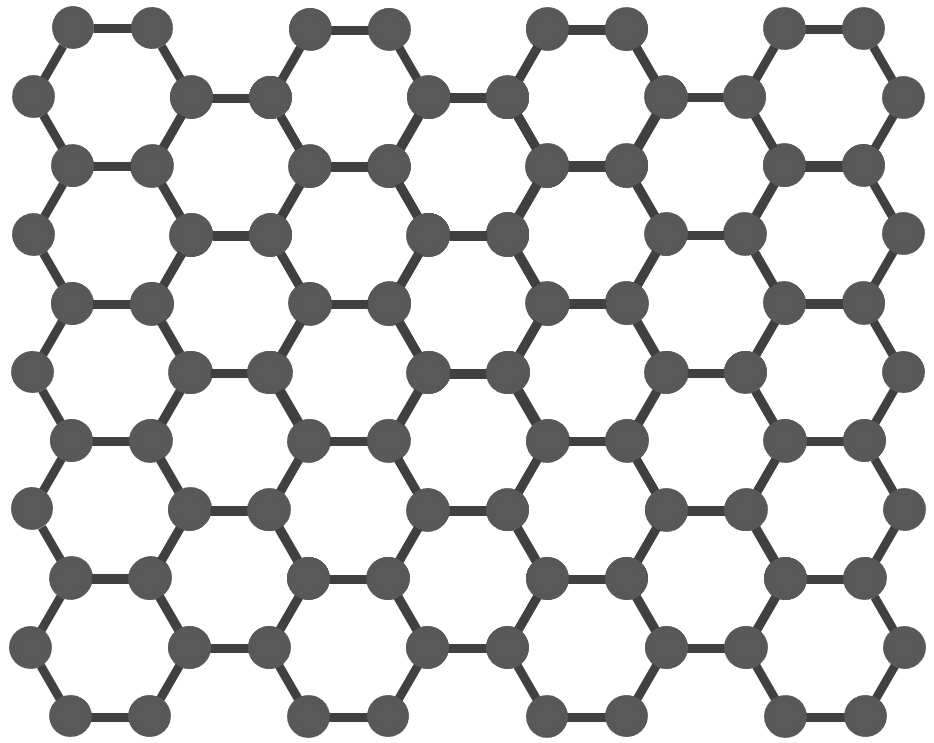
\includegraphics[height=4cm,width=5cm]{figs/graphene_honeycomb}
		\caption[Graphene honeycomb lattice]{Graphene: a layer of carbon atoms in a honeycomb lattice.}
		\label{fig:graphene_honeycomb}
	\end{minipage}
%\end{figure}
%\begin{figure}[ht]
	\qquad
	\begin{minipage}[b]{0.45\linewidth}
		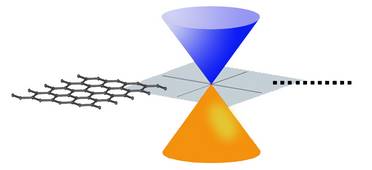
\includegraphics[height=4cm,width=6cm]{figs/graphene_bandgap}
		\caption[Bandgap of graphene]{One of the most unusual features of graphene is that its conduction and valence bands meet at a point, meaning that in single-layer graphene there is no band gap (figure obtained from \cite{Berkley_Online2009})}
		\label{fig:graphene_bandgap}
	\end{minipage}
\end{figure}

\subsection{Band Structure of Graphene}\label{subsec:graphene_bandstructure}
\noindent Despite its impressive properties, the main drawback of graphene is its lack of bandgap. As this became known, the prospect of using graphene for the fabrication to \acp{IC} became unlikely. In graphene the conduction and valence bands touch at a single point as shown in fig.~\ref{fig:graphene_bandgap} \cite{Wallace_PhysRev1947}. Ultimately, the lack of a bandgap means that the current on/off ratio is low and is unappealing for logical circuit applications \cite{Xu_ChemRev2013}. However, graphene exhibits some interesting properties as a result of having no bandgap, particularly as it pertains to its optical properties. The material's band structure allows for absorption of light over a large range of the electromagnetic spectrum, ranging from infrared ($<1.65\unita{eV}$) to ultraviolet ($>3.2\unita{eV}$), offering potential electronic-photonic device applications \cite{Xia_NatureNano2009,Wang_Science2008,Geim_NatureComm2011}. Since a direct use in logical circuits is not practical researchers have moved on to look for `\td materials beyond graphene.' Several attempts at some derivatives of graphene-like materials have been studied, but for the most part they do not seem promising for use in logical circuits \cite{Takeda_PhysRev1994,Cahangirov_PhysRevLett2009}. As of late, research has been concentrated on \td materials, namely transition methal dichalcogenides, as a candidate for applications in \acp{IC}.

\section{\Td Materials: Transition Metal Dichalcogenides}\label{sec:tmds}
Commonly referred to \td materials beyond graphene, \ac{TMD} have garnered much interest. \acp{TMD} were studied previously, however, they have gained renewed interest due to their properties \cite{Frindt_Royal1963,Fivaz_PhysRev1967,Mattheiss_PhysRevB1973,Wilson_AdvPhys1969}. \acp{TMD} consist of hexagonal layers of metal (\ch{M}) atoms in between two laters chalcogen (\ch{X}) atoms (see fig.~\ref{fig:tmd_hexagonal}, such that the stoichiometry of the material is \ch{MX2} \cite{Xu_ChemRev2013}. The material is dependent on the type of transition metal, typically one of: \ac{Mo}, \ac{W}, \ac{Nb}, \ac{Re}, \ac{Ni}, or \ac{V}, and two chalcogen atoms, typically one of: \ac{S}, \ac{Se}, or \ac{Te} \cite{Wilson_AdvPhys1969,Wells_Oxford1984}. The most commonly studied variations of \acp{TMD} are \ac{MoS2}, \ac{WSe2}, and \ac{WS2}. These materials are commonly stacked together involving van der Waals interactions between adjacent sheets and covalent bonding within each individual sheet (see fig.~\ref{fig:tmd_layer}) \cite{Xu_ChemRev2013}.
\begin{figure}[ht]
	\centering
	\begin{minipage}[b]{0.45\linewidth}
		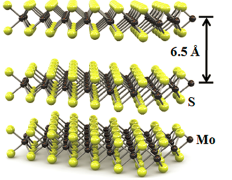
\includegraphics[height=4cm,width=6cm]{figs/tmdlayered}
		\caption[Layered \acs{TMD} diagram]{The atomic structure of a layered \acs{TMD}, depicting \acs{MoS2}. Each sheet is composed of three atoms with \ch{Mo} sandwiched in between two \acs{S} atoms, \acs{S}-\acs{Mo}-\acs{S}. (Figure obtained from \cite{Kis_NatureNano2011})}
		\label{fig:tmd_layer}
	\end{minipage}
	\qquad
	\begin{minipage}[b]{0.45\linewidth}
		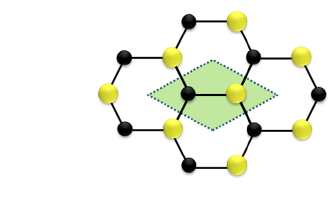
\includegraphics[height=4cm,width=6cm]{figs/tmdhexagonal}
		\caption[Hexagonal lattice of \acs{TMD}]{Top view of a \acs{TMD} (\acs{MoS2}) lattice. (Figure obtained from \cite{Kis_NatureNano2011})}
		\label{fig:tmd_hexagonal}
	\end{minipage}
\end{figure}
\noindent \acp{TMD} exhibit a wide variety of properties, including either being a metal or insulator, and displaying the topological insulator effect, superconductivity, and thermoelectricity \cite{Lang_ACSnano2012,Zhang_AdvMat2012,Xie_AppPhysLett2009,Gamble_JournChemPhys1975}.

\subsection{Properties of Commonly Used \acp{TMD}}\label{subsec:tmd_properties}
\noindent As stated in sec.~\ref{subsec:graphene_bandstructure}, one important propert as it pertains to applications for logical circuits is the material's band structure. One of the main reasons \acp{TMD} have been so extensively studied lately is due to the fact that, unlike graphene, they do exhibit a band gap. The band gaps in some commonly used \acp{TMD} is interesting because of the transition from an indirect to a direct band gap as the layered thickness decreases. Fig.~\ref{fig:mos2_bandstructure} illustrates this, for bulk and few-layer \acs{MoS2} there is an indirect band gap while for monolayer \acs{MoS2} there is a direct band gap. This unusual structure results in some unique optical and properties.
\begin{figure}[ht]
	\centering
	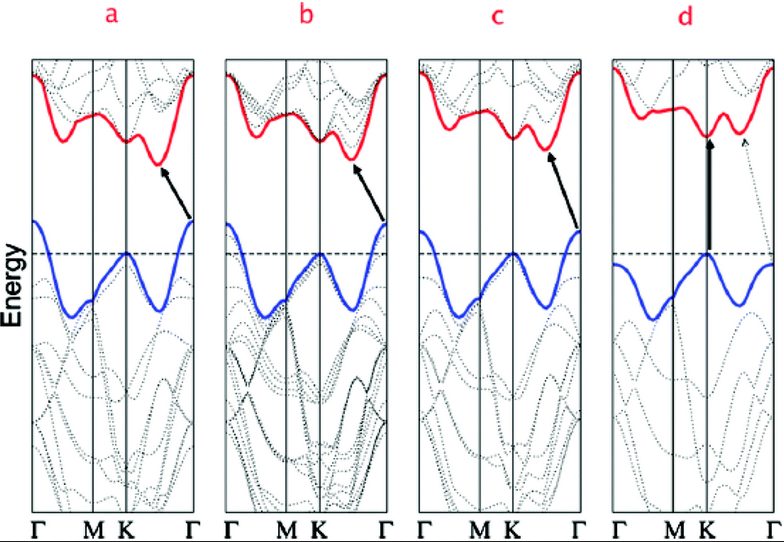
\includegraphics[height=5cm,width=8cm]{figs/mos2_bandstructure}
	\caption[Band structures of \acs{MoS2}]{Calculated band structures of (a) bulk \acs{MoS2}, (b) four-layer \acs{MoS2}, (c) bilayer \acs{MoS2}, and (d) monolayer \acs{MoS2}. Here the solid arrows indicate the lowest energy transitions. (Taken from \cite{Lee_Nanoscale2014}, originally appeared in \cite{Splendiani_Nanolett2010})}
	\label{fig:mos2_bandstructure}
\end{figure}
 
 \begin{table}[ht]
	\centering
	\begin{threeparttable}
	\begin{tabular}{c c c}
		\hline\hline
		2D material & theoretical $E_g\,(\mathrm{eV})$ & experimental $E_g\,(\mathrm{eV})$ \\ [0.5ex]
		\hline
		graphene & 0 & 0 \\
		bilayer graphene & 0 & 0\\
		bulk $h$-\ch{BN} & - & 5.97 \cite{Kubota_Science2007}\\
		monolayer $h$-\ch{BN} & - & 6.07 \cite{Kim_NanoLett2011}\\
		few layer (2-5) $h$-\ch{BN} & - & 5.92 \cite{Song_NanoLett2010}\\
		bulk \acs{MoS2} & 1.2\tnote{a,b}\,\,\,\,\, \cite{Mak_PhysRevLett2010,Gourmelon_Solar1997} & 1.0-1.29\tnote{b}\,\,\, \cite{Mak_PhysRevLett2010,Gourmelon_Solar1997}\\
		monolayer \acs{MoS2} & $\sim 1.90$\tnote{a,c}\,\,\,\,\, \cite{Fortin_JournChemSolids1982} & $\sim 1.90$\tnote{b}\,\,\, \cite{Fortin_JournChemSolids1982}\\
		bulk \acs{WS2} & $\sim 1.30$\tnote{a,b}\,\,\,\,\, \cite{Mak_PhysRevLett2010,Kuc_PhysRevB2011} & $\sim 1.35$\tnote{c}\,\,\, \cite{Mak_PhysRevLett2010,Kuc_PhysRevB2011}\\
		monolayer \acs{WS2} & $\sim 2.10$\tnote{a,c}\,\,\,\,\, \cite{Ma_JournChemPhys2011} &-  \\
		\hline
		\label{table:band_gaps}
	\end{tabular}
	\begin{tablenotes}
		\item[a] Theoretical calculations based on first-principles calculations using \ac{DFT}.
		\item[b] Indirect band gap semiconductor.
		\item[c] Direct band gap semiconductor.
	\end{tablenotes}
	\caption[Band gaps of typical \acp{TMD} and other materials]{Summary of the band gaps of typical monolayer, bilayer, and bulk \acp{TMD} and $h$-\ch{BN} materials. Table adapted from ref.~\cite{Xu_ChemRev2013}.}
	\end{threeparttable}
\end{table}

\subsection{Current State of TMDs}\label{subsec:tmd_current_state}
